\documentclass{cup-pan}
\usepackage{blindtext}
\usepackage{comment}
\usepackage{setspace}
\spacing{1.15}
\renewcommand*\contentsname{Summary of the contents}
\subsectionfont{\color{PANDarkBlue}}

\title{Practical Coursework,\\ Video Game FanArt, \\ The Legend of Zelda: Breath of the Wild.}

\author{Jesus Jimenez Montero}

\affil[1] {Informática Básica, VJ1202}
\affil[2] {Expresión Artística, VJ1204}
\affil[3] {Inglés Moderno, VJ1205}

%% Corresponding author
\corrauthor{Jesús Jiménez Montero}

%% Abbreviated author list for the running footer
\runningauthor{Jesus JM}

\addbibresource{refs.bib}

\begin{document}

\maketitle
%\hrule
\textcolor{PANDarkBlue}{\hrule}


\tableofcontents
\newpage
\listoffigures
\newpage

\begin{abstract}
    This document is a practical coursework for the subject, "Informática Básica". It's a fanart of the video game, "The Legend of Zelda: Breath of the Wild". The main goal of this coursework is to adapt the Hero's Quest to the drawings.
    This document will be written in English due to the collaboration with the subject, "Inglés Moderno". 
    And the format of the document is done with the language LaTeX, and the template PAN (Template for submission to Political Analysis).

\end{abstract}

%%______________________________________________________________________________
%%______________________________________________________________________________

\section{Introduction}

    \textcolor{PANDarkBlue}{\large Description of the game}\\
    
    The Legend of Zelda, Breath of the Wild; is a video game exclusive to the Nintendo Switch console, released in 3rd March 2017. 
    Breath of the Wild is an open-world adventure game based on the world of Hyrule, 100 years after the battle that took place where Ganon was sealed in the castle of Hyrule with Zelda protecting the seal. Link is almost defeated on this battle and goes to a deep sleep.
    
    After 100 years as previously mentioned, he's woken up by a distant Zelda from its dormancy and goes out of the cave he was staying at, greeted by a distant and sinister Hyrule Castle. And the adventure can begin!\\
    
    \textcolor{PANDarkBlue}{\large Adaptation of the hero's quest}\\
    One of the requirements for this coursework was to adapt the Hero's Quest to the drawings.
    To make my drawings accomplish this task, I used the key points of Link's Adventure, being:\\
        \begin{enumerate}
            \item After the extended tutorial where Link's gets its paraglider to get down the plateau where the game begins and one of the first things the player does is look to the Dueling Peaks, one of the key points on the game, where Link discovers its true quest.\\
            \item Where the player gains its confidence to destroy a Guardian, whose quest is to keep out intruders from key areas. This also a key point of the game because destroying a guardian means you are one step closer to defeating Ganon. \\
            \item ESTE PUNTO HACE FALTA COMPLETARLO YA QUE NO TENGO NINGUN DIBUJO, tiene que ser del ultimo fan art, en concreto de un key point de la historia que sea ultimo del juego. \\
        \end{enumerate}

%%______________________________________________________________________________
%%______________________________________________________________________________

\section{Reference images}

    For the images used in the project, I used a combination of images from the game (to make the fan arts as accurate as possible), images from internet and the most important par and 3D renders made in Blender.\\

    \subsection*{Images from the game}
    Beginning with the captures of the game, for the Dueling Peaks, I used the following image:\\
    \begin{figure}[H]
        \includegraphics[width=\textwidth]{Imagenes/Referencias/article_img03_1.jpg}
        \caption{Image reference of the Dueling Peaks}
    \end{figure}
    This image gave me the point of reference to create the player on the hill. 

    And this image: 
    \begin{figure}[H]
        \includegraphics[width=\textwidth]{Imagenes/Referencias/Dueling_Peaks.png}
        \caption{The Dueling Peaks with the bridge near the enemy camp}
    \end{figure}
    This image was also very important in the creation of the fan art, because it was the biggest reference point of the Dueling Peaks.\\

    \subsection*{3D Renders}
    I also used 3D renders to make the fan arts, because my area of expertise is 3D, and I wanted to take advantage of this.
    So first, a simple blocks rig
    (\footnote{Rig made by 
    \href{https://hozq3d.gumroad.com/l/Blocks}{hozq3d}}) 
    was used to pose the character: 
    \begin{figure}[H]
        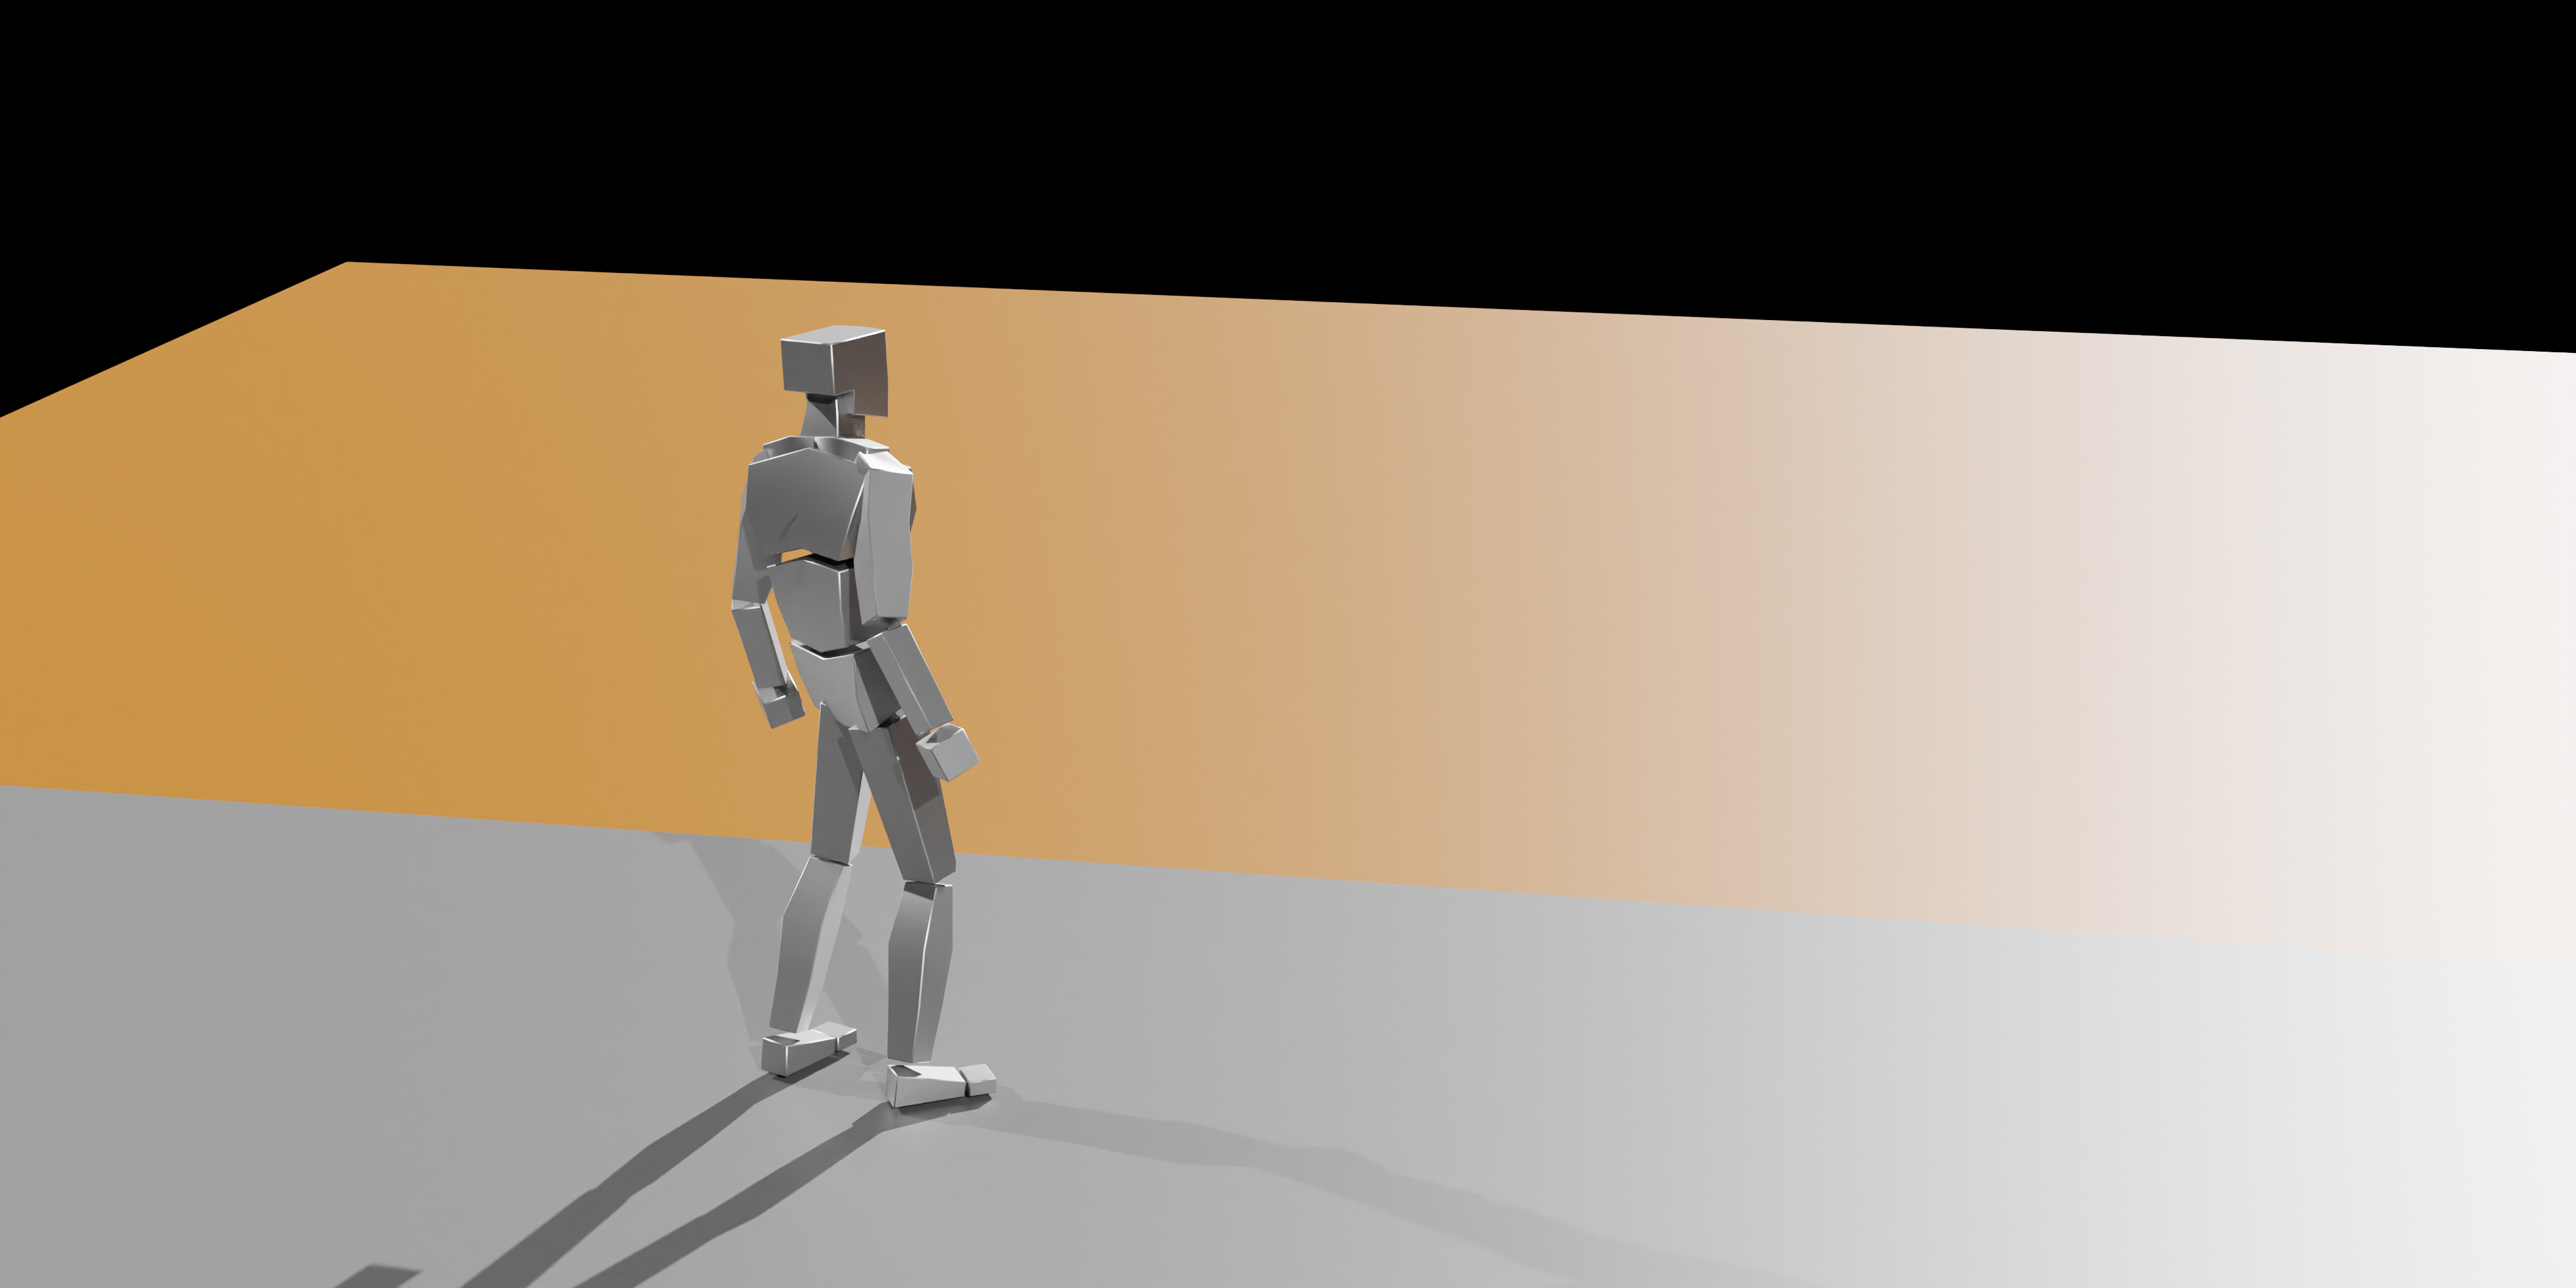
\includegraphics[width=\textwidth]{Imagenes/Referencias/renefernce_3d_3.png}
        \caption{Blocks rig}
    \end{figure}

    And then, a rig of Zelda was used to pose the final character and have more detail:    
    (\footnote{Rig made by 
    \href{https://www.youtube.com/watch?v=1EUcGBMVRbA}{Soranin} and ported to Blender by  
    \href{https://twitter.com/mehaloArt/status/1528197222751383552?s=20}{mehaloArt}})

    \begin{figure}[H]
        \includegraphics[width=\textwidth]{Imagenes/Referencias/ref_zelda.png}
        \caption{Zelda rig}
    \end{figure}

    The Zelda Rig was also used in combination with another rig, which was a Guardian 
    (\footnote{Rig made by 
        \href{https://sketchfab.com/3d-models/guardian-zelda-botw-fan-art-990a6a9434c849329360ea1ef9078895}{NinKorr3D}}), to make the final fanart.
    \begin{figure}[H]
        \includegraphics[width=\textwidth]{Imagenes/Referencias/referencia art 2.png}
        \caption{Zelda and the Guardian Rig}
    \end{figure}

    The usage of manually created 3D renders allowed for a much diverse expression of the fan arts, allowing a preview of how the final fan art would look like and facilitating the creation process.\\

    For the most part, the thematic of the fan arts was to create an impression on the spectator, make them feel something. For example, on the first fan art, I want the spectator to feel the same feeling that the player felt when it saw the Dueling Peaks for the first time. \\

    And on the second fan art, I want the spectator to feel the same feeling that the player has when it destroyed the first Guardian.

%%______________________________________________________________________________
%%______________________________________________________________________________

\section{Analysis of formal elements of a concept art}
    \begin{figure}[H]
       \includegraphics[width=\textwidth]{Imagenes/Referencias/conceptart_a_analizar_2.png}
        \caption{Concept art to analyze}
    \end{figure}

        \subsection{Perspective}
            \begin{figure}[H]
                \includegraphics[width=\textwidth]{Imagenes/Referencias/Analisis_ConceptArt/horizonte.png}
                \caption{Horizon line.}
            \end{figure}

            No vanishing point, organic composition

        \subsection{Composition}
            \begin{figure}[H]
                \includegraphics[width=\textwidth]{Imagenes/Referencias/Analisis_ConceptArt/tercios.png}
                \caption{Rule of Thirds}
            \end{figure}

            \begin{figure}[H]
                \includegraphics[width=\textwidth]{Imagenes/Referencias/Analisis_ConceptArt/recorridovisual.png}
                \caption{Visual Paths.}
            \end{figure}

            \begin{figure}[H]
                \includegraphics[width = \textwidth]{Imagenes/Referencias/Analisis_ConceptArt/puntos interes.png}
                \caption{Points of interest.}
            \end{figure}

            \begin{figure}[H]
                \includegraphics[width=\textwidth]{Imagenes/Referencias/Analisis_ConceptArt/balanza.png}
                \caption{Weight Balance.}
            \end{figure}

        \subsection{Chiaroscuro}
            \begin{figure}[H]
                \includegraphics[width=\textwidth]{Imagenes/Referencias/Analisis_ConceptArt/claroscuro.png}
                \caption{Chiaroscuro.}
            \end{figure}

            \begin{figure}[H]
                \includegraphics[width=\textwidth]{Imagenes/Referencias/Analisis_ConceptArt/pixel.png}
                \caption{Pixelizated Chiaroscuro.}
            \end{figure}

            \begin{figure}[H]
                \includegraphics[width=\textwidth]{Imagenes/Referencias/Analisis_ConceptArt/recorrido luz.png}
                \caption{Light Path.}
            \end{figure}

        \subsection{Color}

             \begin{figure}[H]
                \includegraphics[width=\textwidth]{Imagenes/Referencias/Analisis_ConceptArt/paleta.png}
                \caption{Color Palette.}
            \end{figure}

            \begin{figure}[H]
                \includegraphics[width=\textwidth]{Imagenes/Referencias/Analisis_ConceptArt/tonalidad.png}
                \caption{Color Tonality.}
            \end{figure}

            \begin{figure}[H]
                \includegraphics[width=\textwidth]{Imagenes/Referencias/Analisis_ConceptArt/contrast.png}
                \caption{Color Contrast.}
            \end{figure}

%%______________________________________________________________________________
%%______________________________________________________________________________

\newpage
\section{First Illustration}
    \subsection{Line art and sketches}

        The first fan art was the most difficult to make, because it was the first time I made a fan art and I didn't know how to start. So I started with a simple sketch of the Dueling Peaks. 
        I also used the Blocks Rig previously mentioned to quickly pose a character.\\
        \begin{figure}[H]
            \includegraphics[width=\textwidth]{Imagenes/Fanart1/Boceto_Lineart/0 Imagen de partida.png}
            \caption{First sketch of the Dueling Peaks.}
        \end{figure}

        On the first iteration, I used the previous art on the “Composition I” assignment, by using images from the game and reality to make a quick sketch of how the art would look like.\\
        \begin{figure}[H]
            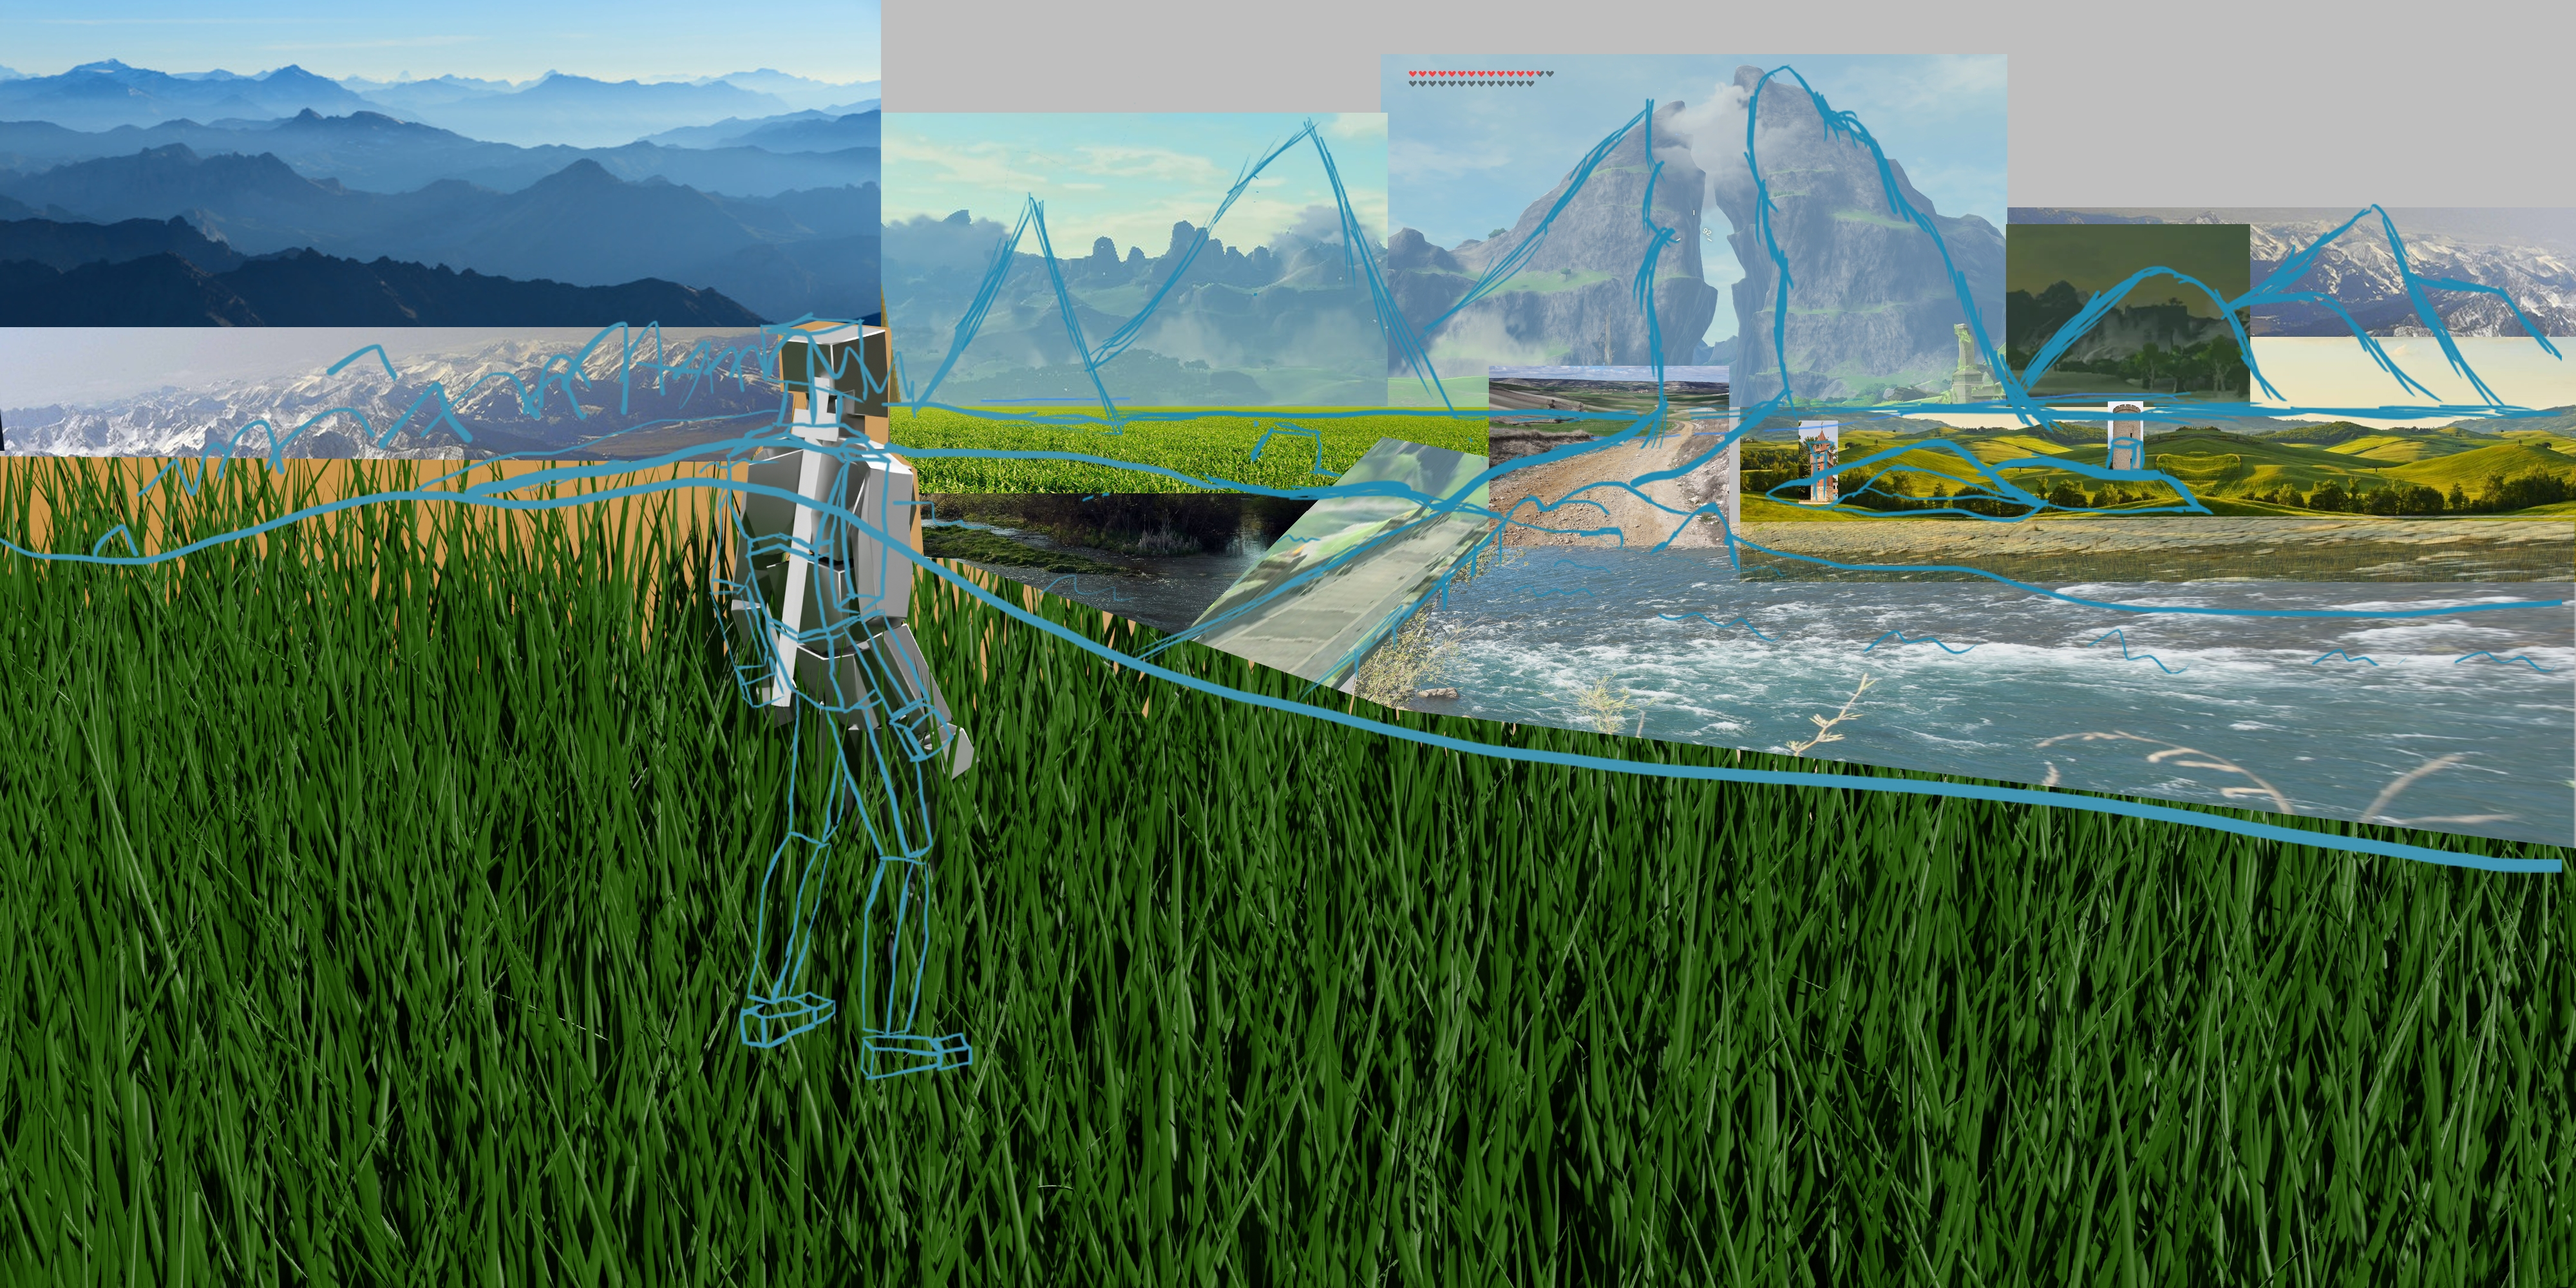
\includegraphics[width=\textwidth]{Imagenes/Fanart1/Boceto_Lineart/1a_Iteracion.jpg}
            \caption{First iteration of the Dueling Peaks, using images as reference.}
        \end{figure}

        On the second iteration, I improved upon the reference images and added more details and tried to make everything consistent in the drawing.\\
        \begin{figure}[H]
            \includegraphics[width=\textwidth]{Imagenes/Fanart1/Boceto_Lineart/2a_iteración.png}
            \caption{Second iteration of the Dueling Peaks.}
        \end{figure}

        On the third iteration, I polished the strokes and added more details to the sketch. Also, I added the grass and some clouds, filling them with a \textit{watery} brush to give it a more \textit{cloudy} feeling.\\
        \begin{figure}[H]
            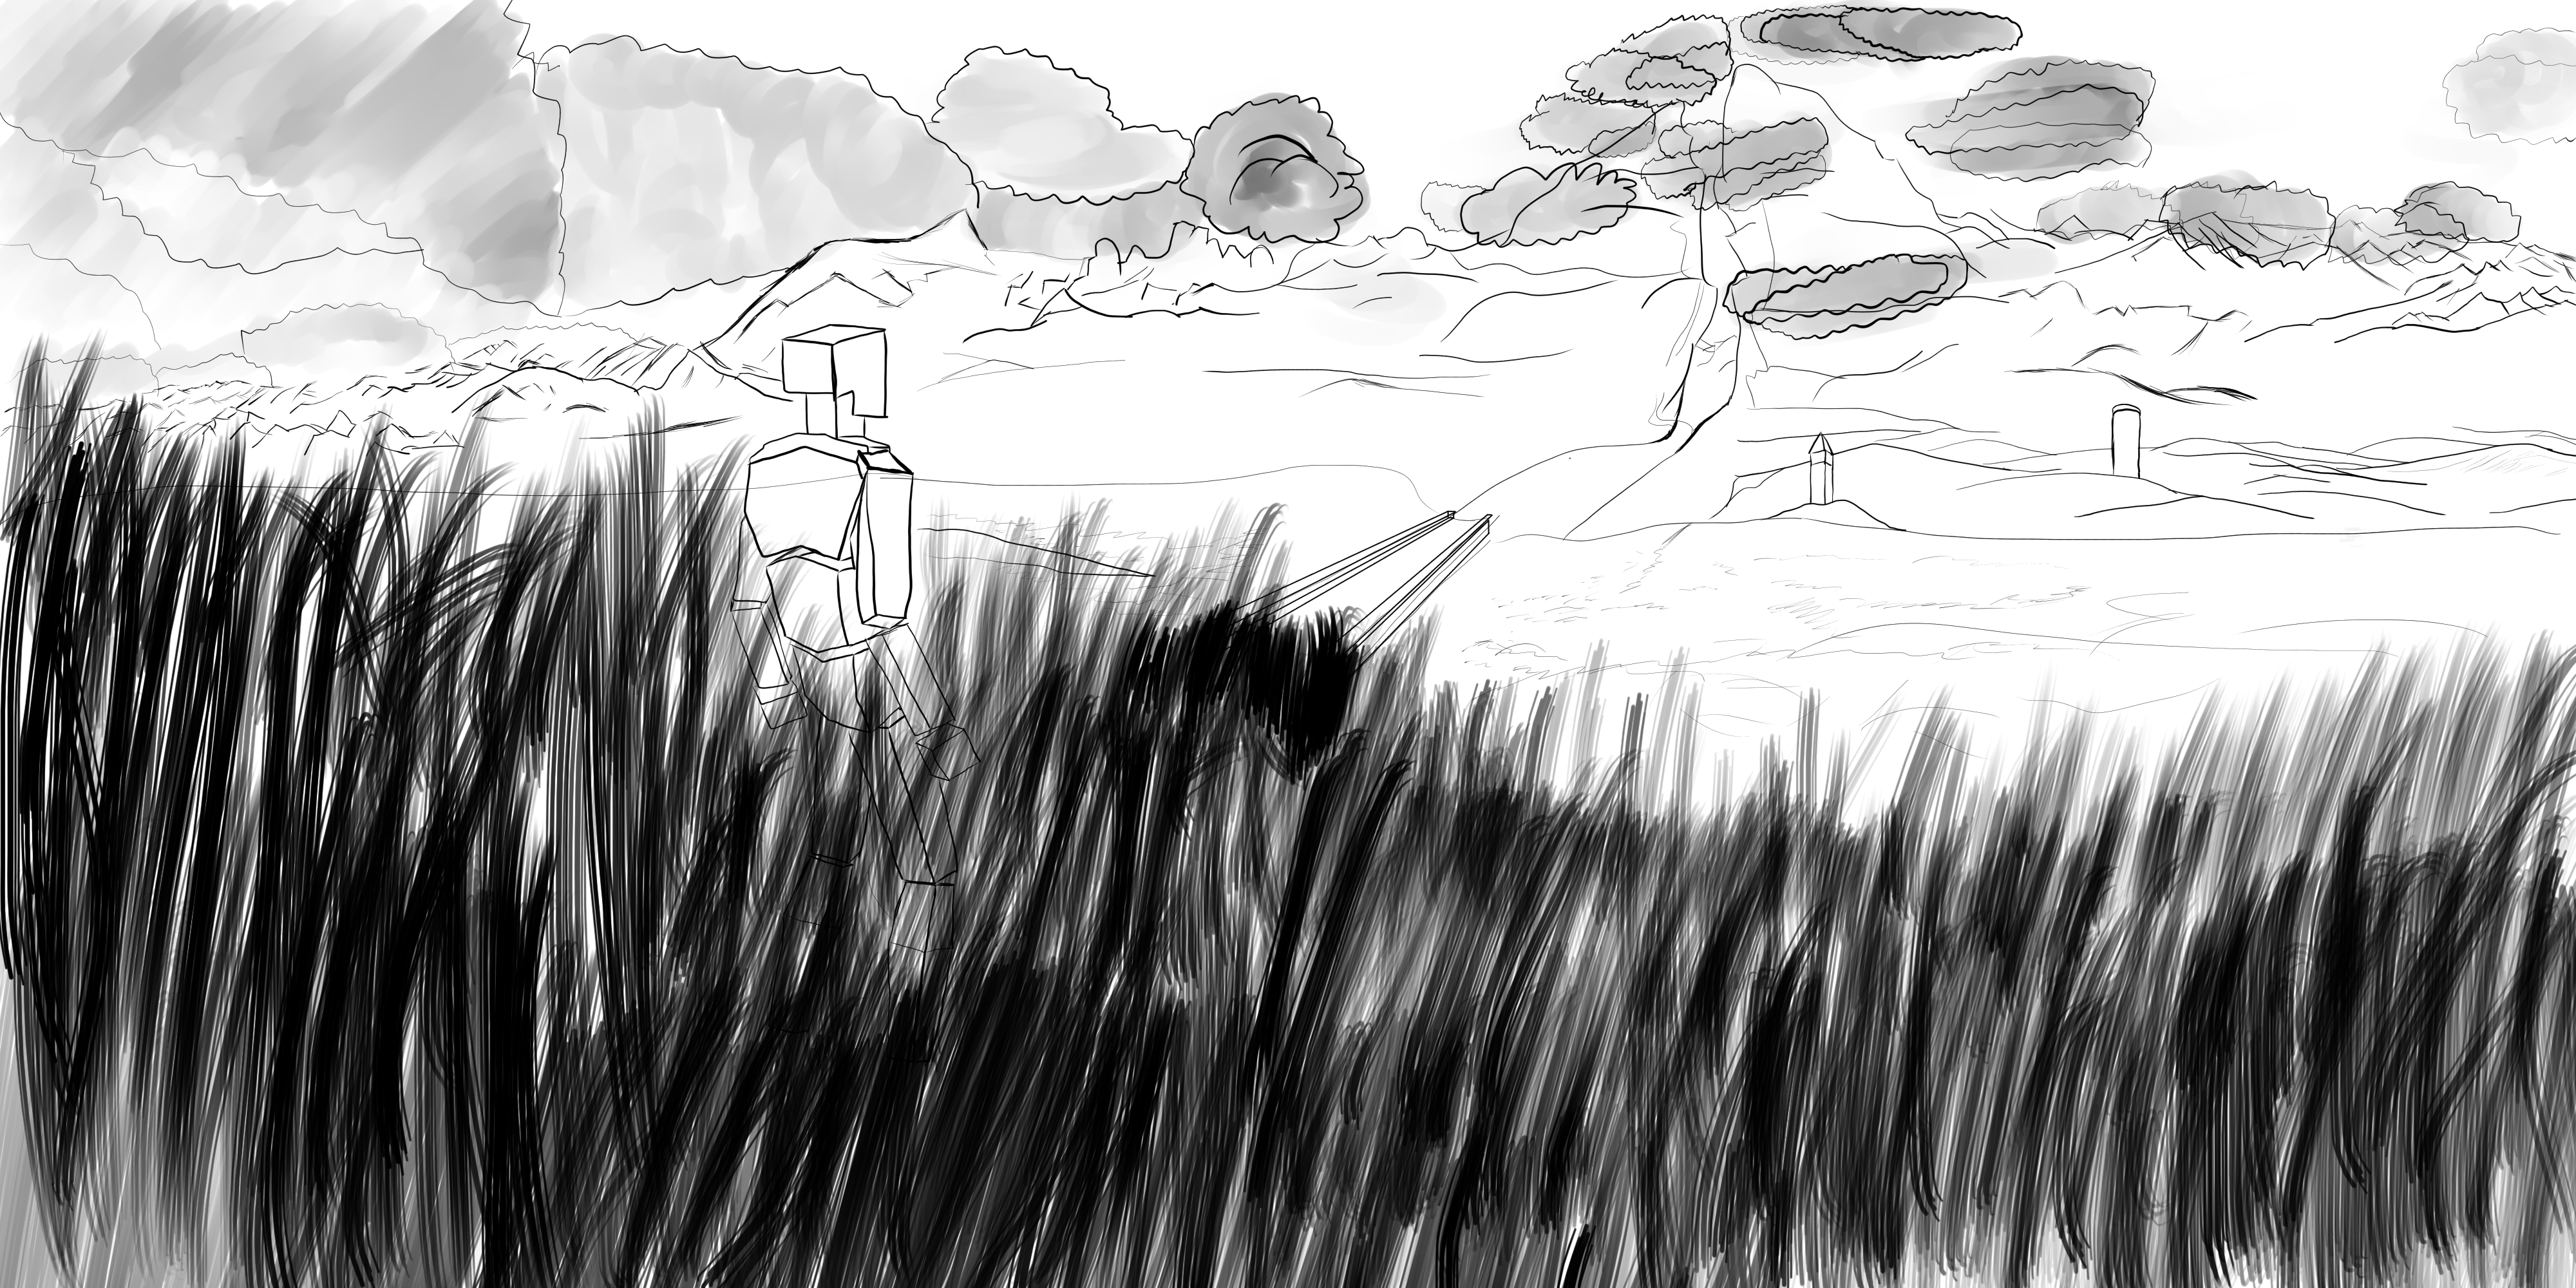
\includegraphics[width=\textwidth]{Imagenes/Fanart1/Boceto_Lineart/3a_iteracion.png}
            \caption{Third iteration of the Dueling Peaks.}
        \end{figure}

        To end with this step, I cleaned up the clouds and removed the coloring. I also changed the blocks rig character for a new one, which was the Zelda Rig.\\
        \begin{figure}[H]
            \includegraphics[width=\textwidth]{Imagenes/Fanart1/Boceto_Lineart/4a_Iteracion.png}
            \caption{Fourth iteration of the Dueling Peaks.}
        \end{figure}

    \subsection{Chiaroscuro}
        Commencing with the chiaroscuro, I sketched how would the blacks and whites would progress naturally to the end of the composition.
        \begin{figure}[H]
            \includegraphics[width=\textwidth]{Imagenes/Fanart1/Claroscuro/Imagen1.png}
            \caption{First iteration of the chiaroscuro.}
        \end{figure}

        On the second iteration, I added more details to the chiaroscuro, making it more consistent with the line art, but the character was done at a later iteration to keep the focus on the scenery.\\
        \begin{figure}[H]
            \includegraphics[width=\textwidth]{Imagenes/Fanart1/Claroscuro/Imagen2.png}
            \caption{Second iteration of the chiaroscuro.}
        \end{figure}

        On the third iteration, I added more details to the chiaroscuro, with some rudimentary shadows and a basic shading, with more clouds added and a basic silhouette of the character.\\
        \begin{figure}[H]
            \includegraphics[width=\textwidth]{Imagenes/Fanart1/Claroscuro/Imagen3.png}
            \caption{Third iteration of the chiaroscuro.}
        \end{figure}

        On the fourth iteration, I added detail to the character and a shadow to it. Also, I added shading to the mountains, character, river and the bridge.This was made to separate everything much better than using just a simple black and white scheme.\\
        \begin{figure}[H]
            \includegraphics[width=\textwidth]{Imagenes/Fanart1/Claroscuro/Imagen4.png}
            \caption{Fourth iteration of the chiaroscuro.}
        \end{figure}

    \subsection{Coloring}
        The coloring part of this fan arts had fewer parts overall, because the chiaroscuro was already done and techniques taught in class were used. Basically, adding a “Color” layer and applying the color from there.\\

        On the first iteration, I added the colors to the chiaroscuro, making the mountains a bit more saturated and adding a bit of color  to the sky and the small forest in the distance.\\
        \begin{figure}[H]
            \includegraphics[width=\textwidth]{Imagenes/Fanart1/Color/I_Iteracion.png}
            \caption{First iteration of the coloring.}
        \end{figure}
        
        On the second iteration, I added colors to the river and the hill. 
        \begin{figure}[H]
            \includegraphics[width=\textwidth]{Imagenes/Fanart1/Color/II_Iteracion.png}
            \caption{Second iteration of the coloring.}
        \end{figure}

        On the third iteration I added some colors to Zelda. 
        \begin{figure}[H]
            \includegraphics[width=\textwidth]{Imagenes/Fanart1/Color/III_Iteracion.png}
            \caption{Third iteration of the coloring.}
        \end{figure}

        And for the last iteration I added a warm and yellowish tone to the sky, to make it look like a sunset.\\
        \begin{figure}[H]
            \includegraphics[width=\textwidth]{Imagenes/Fanart1/Color/IIII_Iteracion.png}
            \caption{Fourth iteration of the coloring.}
        \end{figure}
        
    \subsection{Final Result}
        The final result of the fan art is the following:
        \begin{figure}[H]
            \includegraphics[width=\textwidth]{Imagenes/Fanart1/Color/IIII_Iteracion.png}
            \caption{Final result of the fan art.}
        \end{figure}
        Sadly, due to the grass looking weird when drew and colored, I decided to remove it from the final result.\\

    \subsection{Formal elements of the image}

        \subsubsection{Perspective}

            \begin{figure}[H]
                \includegraphics[width=\textwidth]{Imagenes/Fanart1/Analysis/horizonte.png}
                \caption{Horizon line.}
            \end{figure}

            There's no vanishing point, organic composition

        \subsubsection{Composition}

            \begin{figure}[H]
                \includegraphics[width=\textwidth]{Imagenes/Fanart1/Analysis/reglatercios.png}
                \caption{Rule of Thirds.}
            \end{figure}

            \begin{figure}[H]
                \includegraphics[width=\textwidth]{Imagenes/Fanart1/Analysis/puntosinteres.png}
                \caption{Interset Points.}
            \end{figure}

            \begin{figure}[H]
                \includegraphics[width=\textwidth]{Imagenes/Fanart1/Analysis/recorridovisual.png}
                \caption{Visual Paths.}
            \end{figure}

            \begin{figure}[H]
                \includegraphics[width=\textwidth]{Imagenes/Fanart1/Analysis/balanza.png}
                \caption{Weight Scaling.}
            \end{figure}

        \subsubsection{Chiaroscuro}

            \begin{figure}[H]
                \includegraphics[width=\textwidth]{Imagenes/Fanart1/Analysis/claroscuro.png}
                \caption{Chiaroscuro.}
            \end{figure}

            \begin{figure}[H]
                \includegraphics[width=\textwidth]{Imagenes/Fanart1/Analysis/pixel.png}
                \caption{Pixelizated Chiaroscuro.}
            \end{figure}

            \begin{figure}[H]
                \includegraphics[width=\textwidth]{Imagenes/Fanart1/Analysis/recorridoluz.png}
                \caption{Light Paths.}
            \end{figure}

        \subsubsection{Color}

            \begin{figure}[H]
                \includegraphics[width=\textwidth]{Imagenes/Fanart1/Analysis/paleta.png}
                \caption{Color Palette.}
            \end{figure}

            \begin{figure}[H]
                \includegraphics[width=\textwidth]{Imagenes/Fanart1/Analysis/tonalidad.png}
                \caption{Color Tonality.}
            \end{figure}

            \begin{figure}[H]
                \includegraphics[width=\textwidth]{Imagenes/Fanart1/Analysis/contraste.png}
                \caption{Contrasts.}
            \end{figure}

\newpage
%%______________________________________________________________________________
%%______________________________________________________________________________
\newpage
\section{Second Illustration}

    \subsection{Line art and sketches}

        \begin{figure}[H]
            \includegraphics[width=\textwidth]{Imagenes/Fanart2/Boceto_Lineart/I Iteracion_LineArt.png}
            \caption{First iteration of the line art.}
        \end{figure}
        \begin{figure}[H]
            \includegraphics[width=\textwidth]{Imagenes/Fanart2/Boceto_Lineart/II Iteracion_LineArt.png}
            \caption{Second iteration of the line art.}
        \end{figure}
        \begin{figure}[H]
            \includegraphics[width=\textwidth]{Imagenes/Fanart2/Boceto_Lineart/III Iteracion_2o_FanArt_LineArt.png}
            \caption{Third iteration of the line art.}
        \end{figure}

    \subsection{Chiaroscuro}

        \begin{figure}[H]
            \includegraphics[width=\textwidth]{Imagenes/Fanart2/Claroscuro/I_Iteracion.png}
            \caption{Chiaroscuro.}
        \end{figure}

        \begin{figure}[H]
            \includegraphics[width=\textwidth]{Imagenes/Fanart2/Claroscuro/II_Iteración.png}
            \caption{Chiaroscuro.}
        \end{figure}

        \begin{figure}[H]
            \includegraphics[width=\textwidth]{Imagenes/Fanart2/Claroscuro/III_Iteraion.png}
            \caption{Chiaroscuro.}
        \end{figure}

        \begin{figure}[H]
            \includegraphics[width=\textwidth]{Imagenes/Fanart2/Claroscuro/IIII_Iteracion.png}
            \caption{Chiaroscuro.}
        \end{figure}

        \begin{figure}[H]
            \includegraphics[width=\textwidth]{Imagenes/Fanart2/Claroscuro/IIIII_Iteracion.png}
            \caption{Chiaroscuro.}
        \end{figure}

    \subsection{Coloring}

        \begin{figure}[H]
            \includegraphics[width=\textwidth]{Imagenes/Fanart2/Color/I_Iteracionç.png}
            \caption{Coloring.}
        \end{figure}

        \begin{figure}[H]
            \includegraphics[width=\textwidth]{Imagenes/Fanart2/Color/II_Iteracion.png}
            \caption{Coloring.}
        \end{figure}

        \begin{figure}[H]
            \includegraphics[width=\textwidth]{Imagenes/Fanart2/Color/III_Iteración.png}
            \caption{Coloring.}
        \end{figure}

        \begin{figure}[H]
            \includegraphics[width=\textwidth]{Imagenes/Fanart2/Color/IIII_Iteracion.png}
            \caption{Coloring.}
        \end{figure}

    \subsection{Final Result}

        \begin{figure}[H]
            \includegraphics[width=\textwidth]{Imagenes/Fanart2/Color/IIII_Iteracion.png}
            \caption{Final Result.}
        \end{figure}

    \subsection{Formal elements of the image}
        
        \subsubsection{Perspective}

            \begin{figure}[H]
                \includegraphics[width=\textwidth]{Imagenes/Fanart2/Analysis/horizonte.png}
                \caption{Horizon line.}
            \end{figure}

            There's no vanishing point, organic composition

        \subsubsection{Composition}

            \begin{figure}[H]
                \includegraphics[width=\textwidth]{Imagenes/Fanart2/Analysis/Analysis.png}
                \caption{Rule of Thirds.}
            \end{figure}

            \begin{figure}[H]
                \includegraphics[width=\textwidth]{Imagenes/Fanart2/Analysis/puntos_interes.png}
                \caption{Interset Points.}
            \end{figure}

            \begin{figure}[H]
                \includegraphics[width=\textwidth]{Imagenes/Fanart2/Analysis/recorridos.png}
                \caption{Visual Paths.}
            \end{figure}

            \begin{figure}[H]
                \includegraphics[width=\textwidth]{Imagenes/Fanart2/Analysis/balanza.png}
                \caption{Weight Scaling.}
            \end{figure}

        \subsubsection{Chiaroscuro}

            \begin{figure}[H]
                \includegraphics[width=\textwidth]{Imagenes/Fanart2/Analysis/claroscuro.png}
                \caption{Chiaroscuro.}
            \end{figure}

            \begin{figure}[H]
                \includegraphics[width=\textwidth]{Imagenes/Fanart2/Analysis/pixel.png}
                \caption{Pixelizated Chiaroscuro.}
            \end{figure}

            \begin{figure}[H]
                \includegraphics[width=\textwidth]{Imagenes/Fanart2/Analysis/recorrido luz.png}
                \caption{Light Paths.}
            \end{figure}

        \subsubsection{Color}

            \begin{figure}[H]
                \includegraphics[width=\textwidth]{Imagenes/Fanart2/Analysis/palette.png}
                \caption{Color Palette.}
            \end{figure}

            \begin{figure}[H]
                \includegraphics[width=\textwidth]{Imagenes/Fanart2/Analysis/tonalidad.png}
                \caption{Color Tonality.}
            \end{figure}

            \begin{figure}[H]
                \includegraphics[width=\textwidth]{Imagenes/Fanart2/Analysis/contraste.png}
                \caption{Contrasts.}
            \end{figure}
\newpage
%%______________________________________________________________________________
%%______________________________________________________________________________
\newpage
\section{Third Illustration}

    \subsection{Line art and sketches}

    \subsection{Chiaroscuro}

    \subsection{Coloring}

    \subsection{Final Result}
    \newpage
%%______________________________________________________________________________
%%______________________________________________________________________________
\newpage
\section{Conclusions}

\newpage

\end{document}